\documentclass[utf-8]{ctexart}
\usepackage{a4}
\usepackage{listings}
\usepackage{amsmath,amssymb}
\usepackage{parskip}
\usepackage{graphicx}
\usepackage{indentfirst}%设置锁进
\usepackage[top=2.5cm, left=3cm, right=3cm, bottom=4.0cm]{geometry}

\title{设计文稿}
\author{计92 高敬越 2019011230}

\setlength{\parindent}{2em}

\begin{document}
    \maketitle
    \section{环境}
    \begin{enumerate}
        \item 系统: macOS 10.15.6
        \item Qt版本:Qt 5.15.0 clang 64bit 
    \end{enumerate}
    \section{功能介绍}
    实现了作业要求的所有功能
    \subsection{游戏界面与各个状态}

    \begin{figure}[htb]
        \centering
        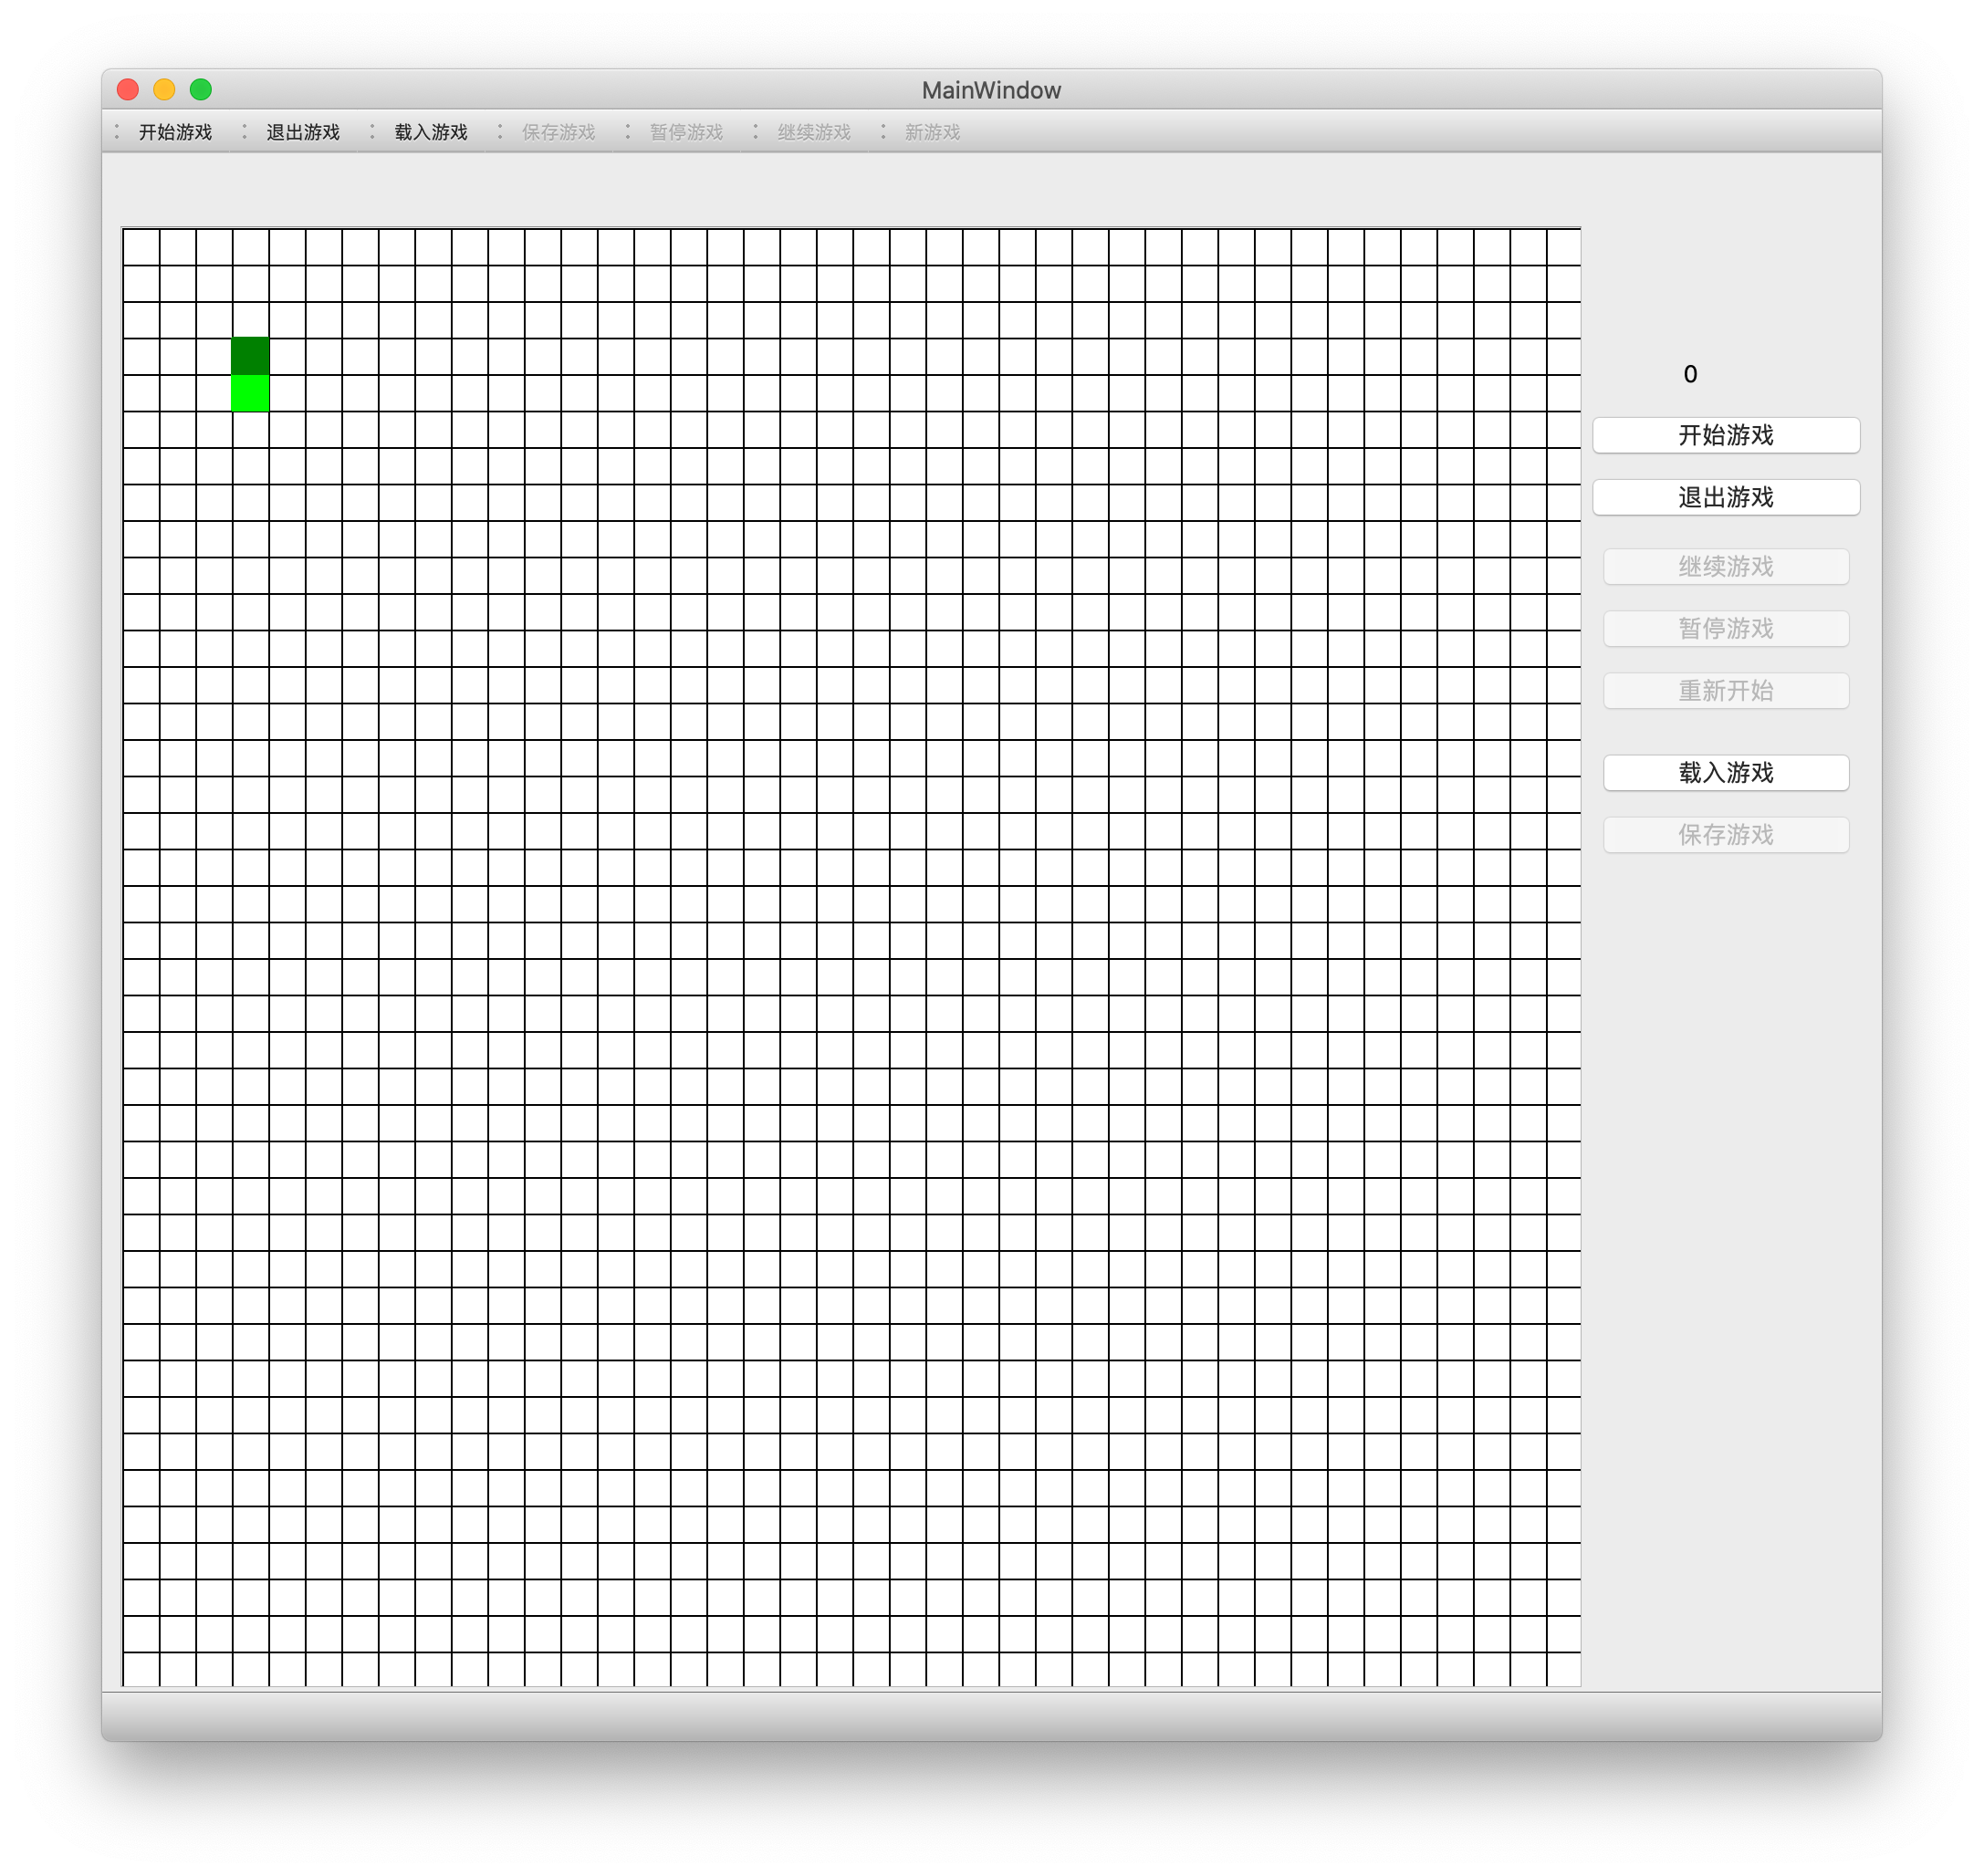
\includegraphics[scale = 0.2]{texsrc/界面.png}
        
\includegraphics[scale = 0.4]{texsrc/菜单栏.png}
        \caption{未开始状态的界面}
        \label{intialized}
    \end{figure}
    \begin{figure}[htb]
        \centering
        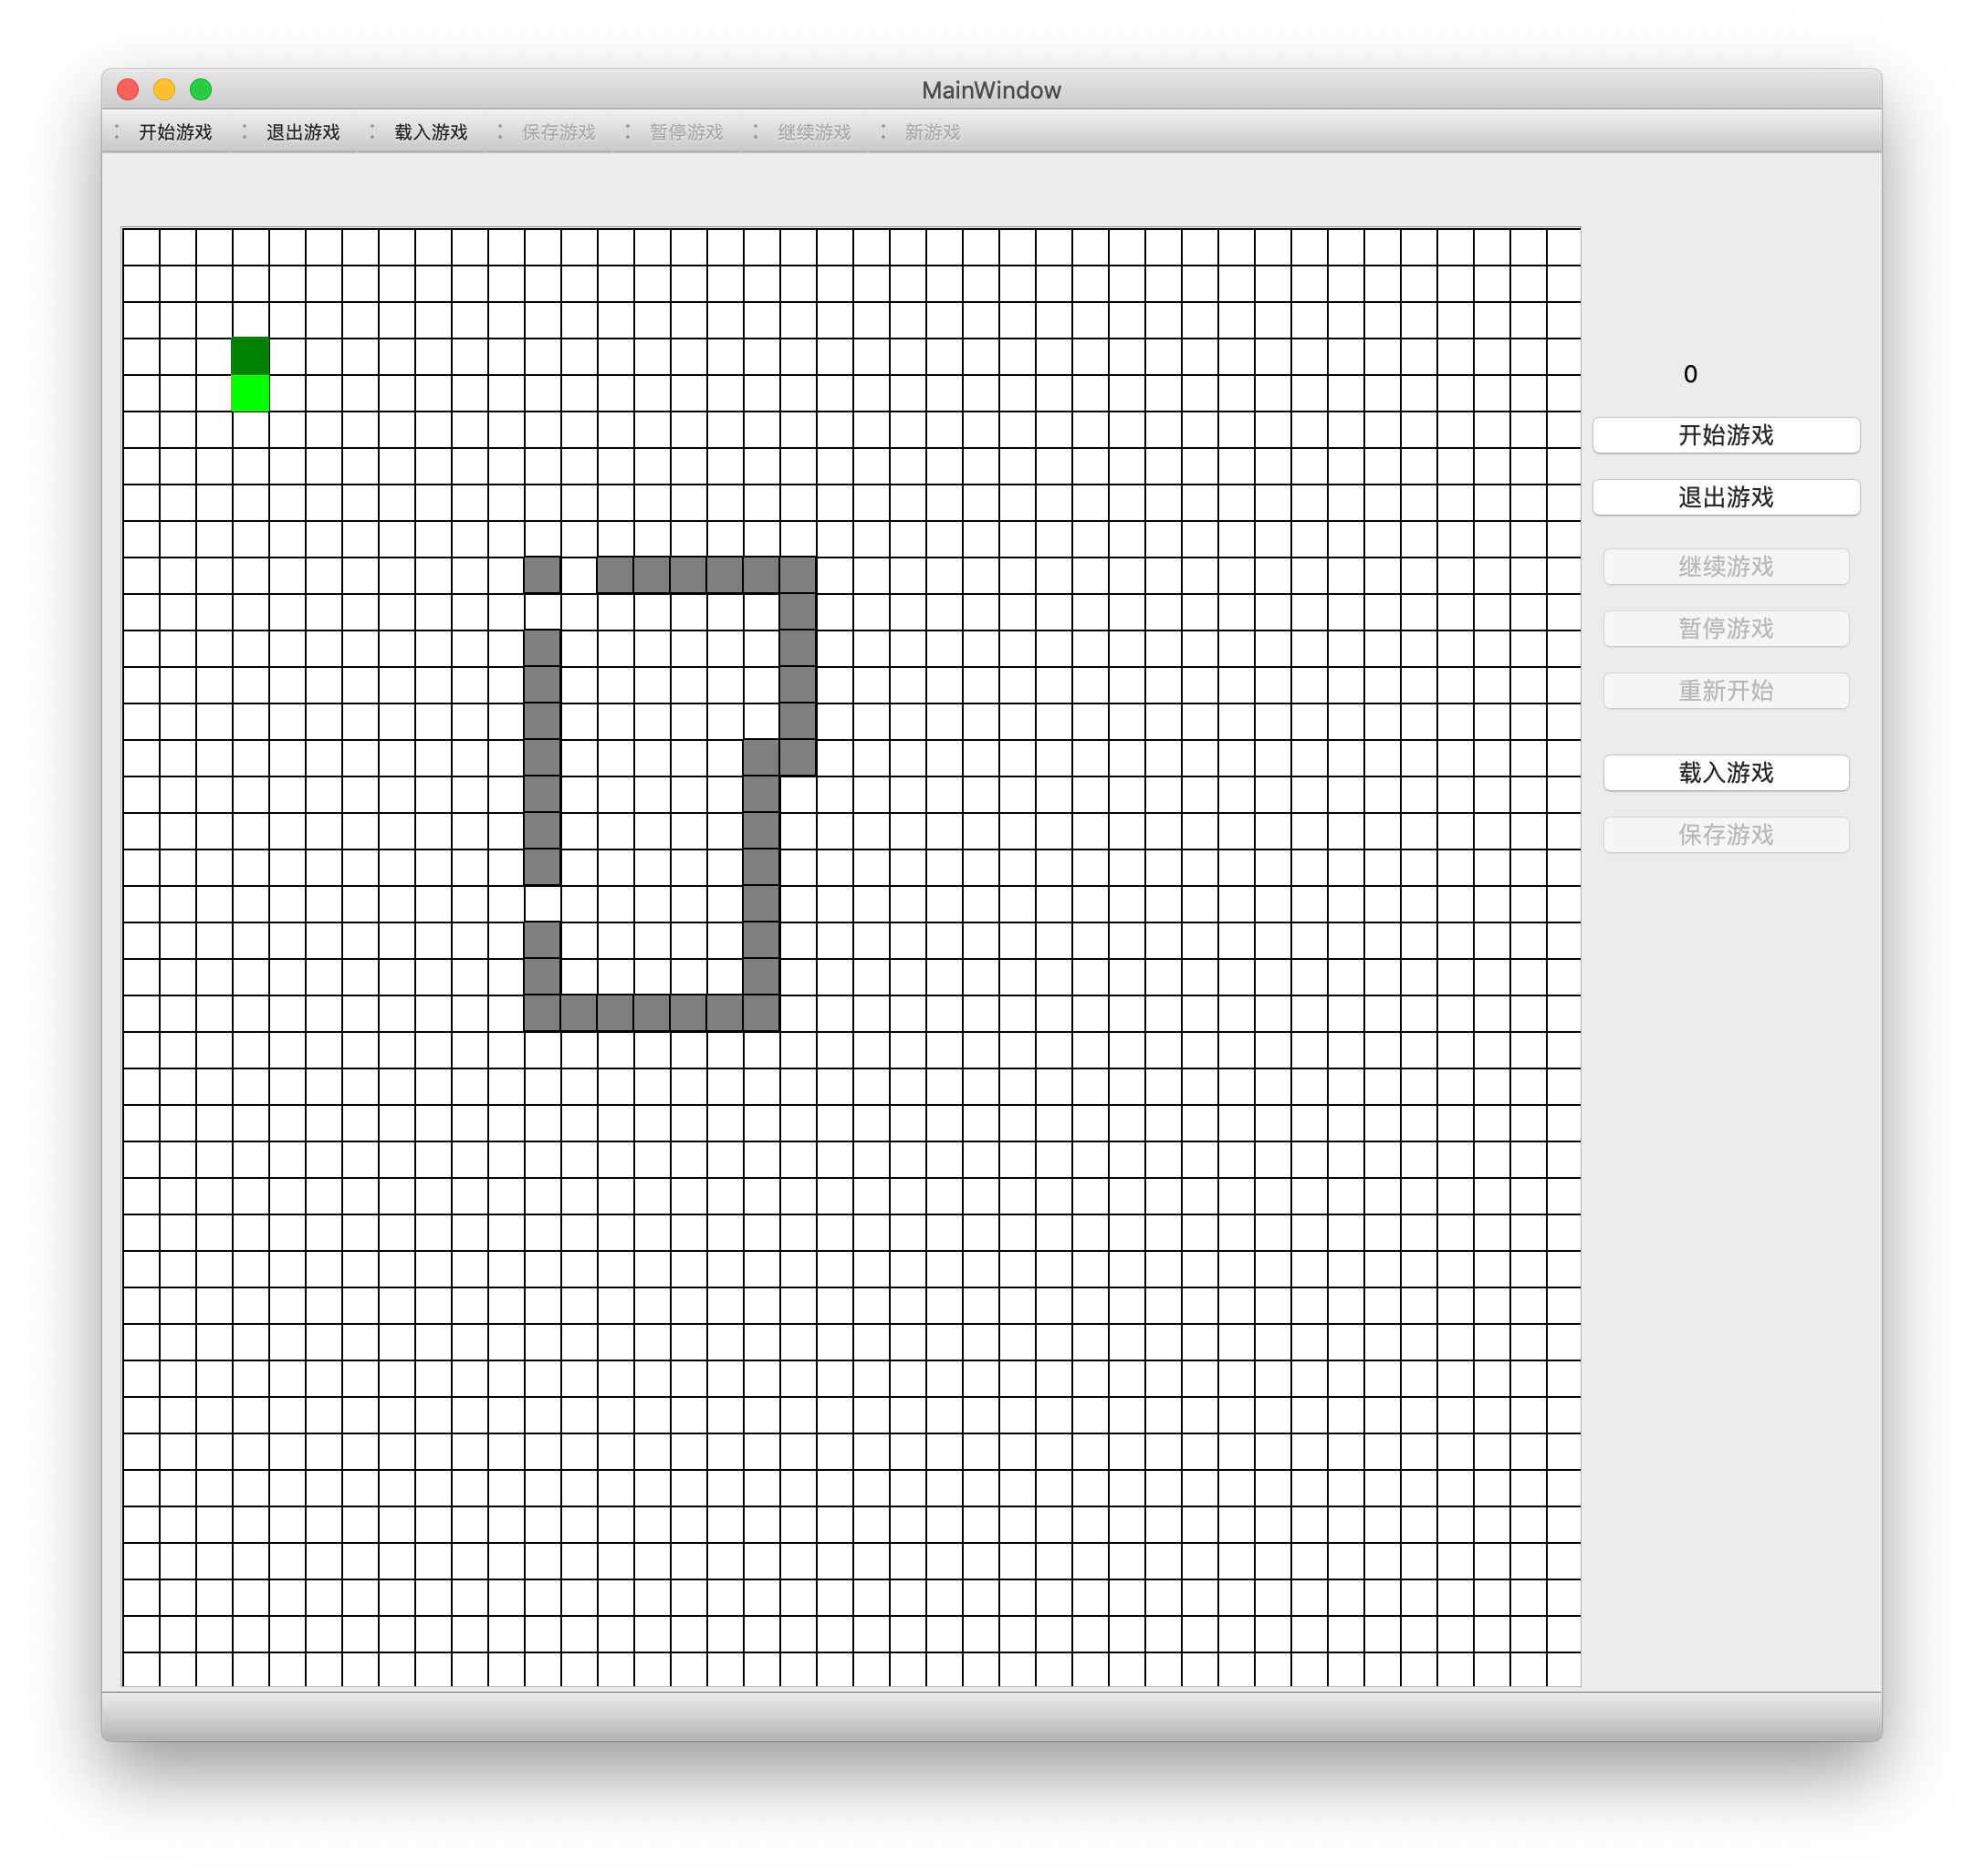
\includegraphics[scale = 0.2]{texsrc/界面+wall.png}
        \caption{点击网格,增加障碍}
        \label{obstacle}
    \end{figure}
    \paragraph{未开始状态} 图1为已初始化、未开始状态时的游戏界面。(由于macOS的特点,应用的菜单栏单独在屏幕最上面,后面的菜单栏就不截了)图1上的图是包含工具栏、按钮、时间展示以及游戏区的主界面,
    图1下为菜单栏。\par 在菜单栏中,“操作”菜单中包含开始游戏、结束游戏两个功能,“保存/载入”菜单中包含保存游戏、载入游戏两个功能,“游戏操作”
    菜单中包含暂停游戏、继续游戏、重新开始三个操作。(具体点开的截图略)\par 在主界面中,最上方一行为工具栏,同样实现了上述的
    所有操作;右侧最上方数字显示时间,大小与蛇走过的距离相同;右侧下方的按钮分别对应了以上所有操作,同时也
    满足了在未开始状态只有开始游戏、退出游戏、载入游戏处于可用状态。主界面中间是40*40格的游戏界面,并初始化了长度为2的蛇(蛇头为深绿色,身体为浅绿色),
    默认运动方向向上。同时在此阶段,可以点击方格来设置障碍,障碍以与各自同样大小的灰色正方形表示(如图2);在增加后,也支持再次点击以消除障碍。
    \par 此状态点击载入游戏可以载入已保存的游戏文件,加载此游戏并进入暂停状态。

    \begin{figure}[htb]
        \centering
        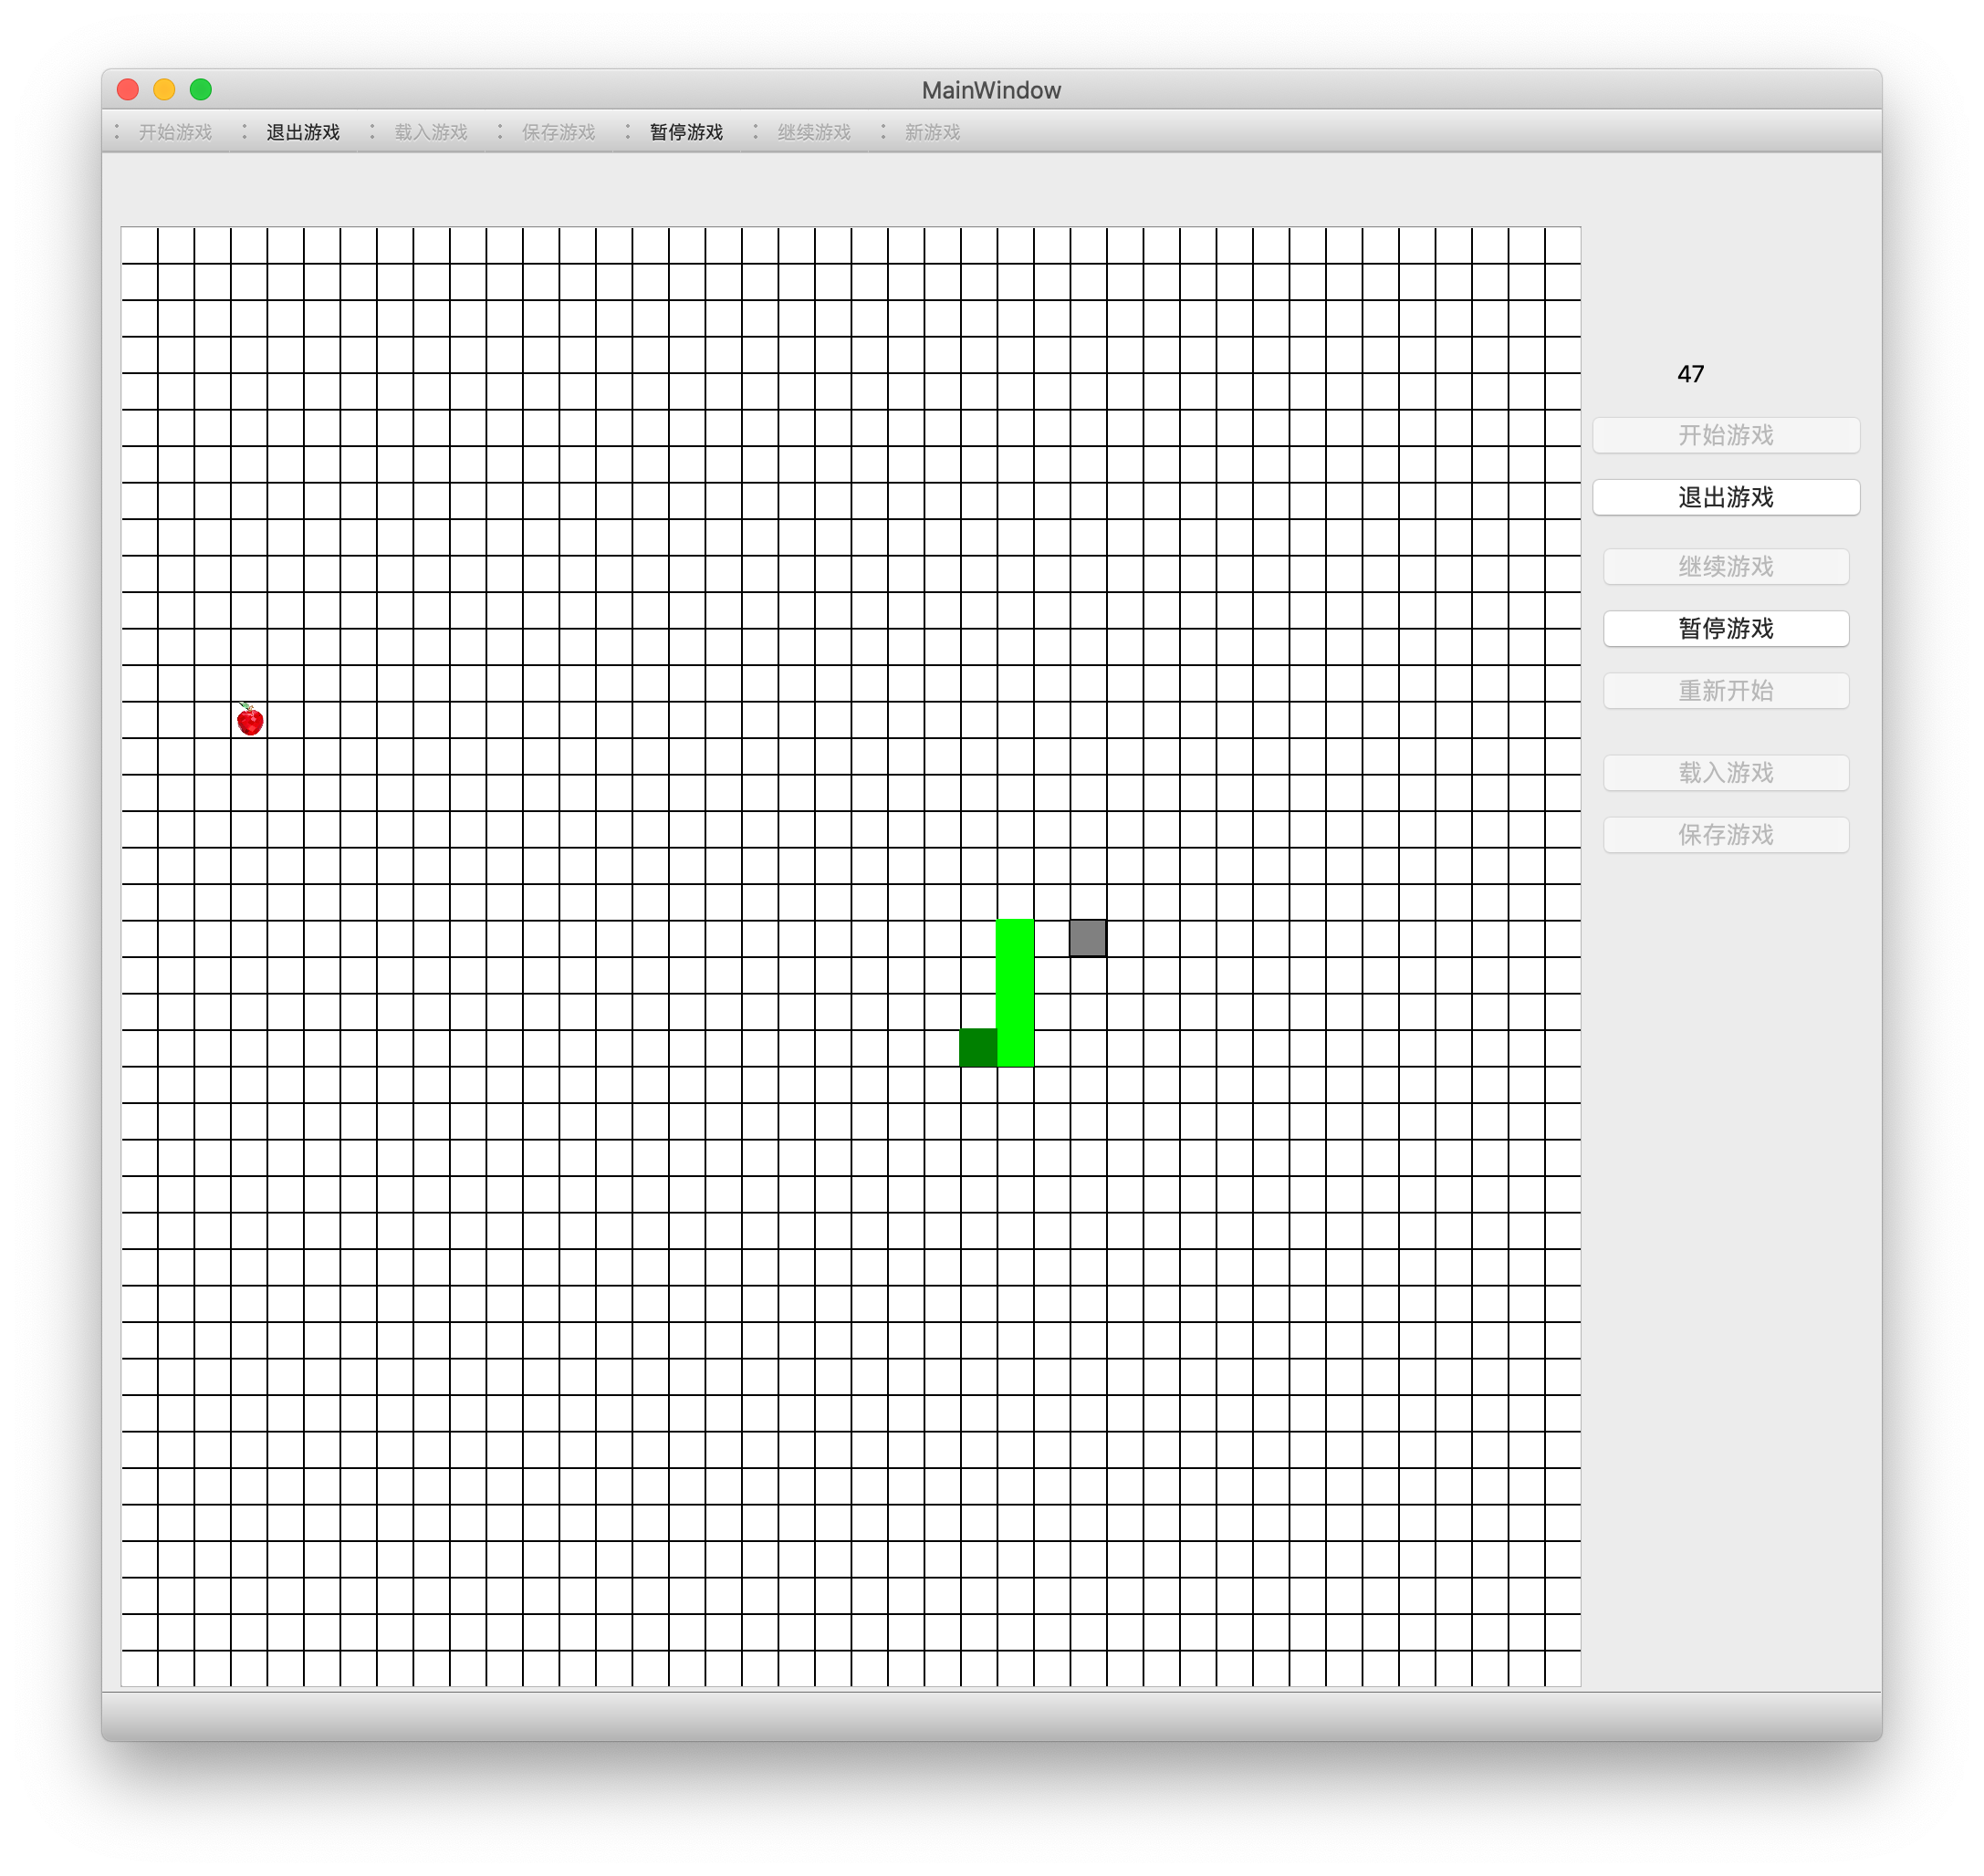
\includegraphics[scale = 0.2]{texsrc/开始游戏.png}
        \caption{游戏状态}
        \label{gaming}
    \end{figure}
    \paragraph{游戏状态} 点击开始游戏后,进入游戏中的状态(如图3)。此时贪吃蛇开始移动,同时随机产生一个食物(图标为小苹果)。此时可以通过方向键调整蛇的运动方向,使其吃水果并避免撞上障碍物。
    在此状态下,只有退出游戏、暂停游戏两个功能可以使用。在吃完苹果后,贪吃蛇将延长3个格,此时尾部不变。
    \par 点击暂停游戏后将进入暂停状态。

    \begin{figure}[htb]
        \centering
        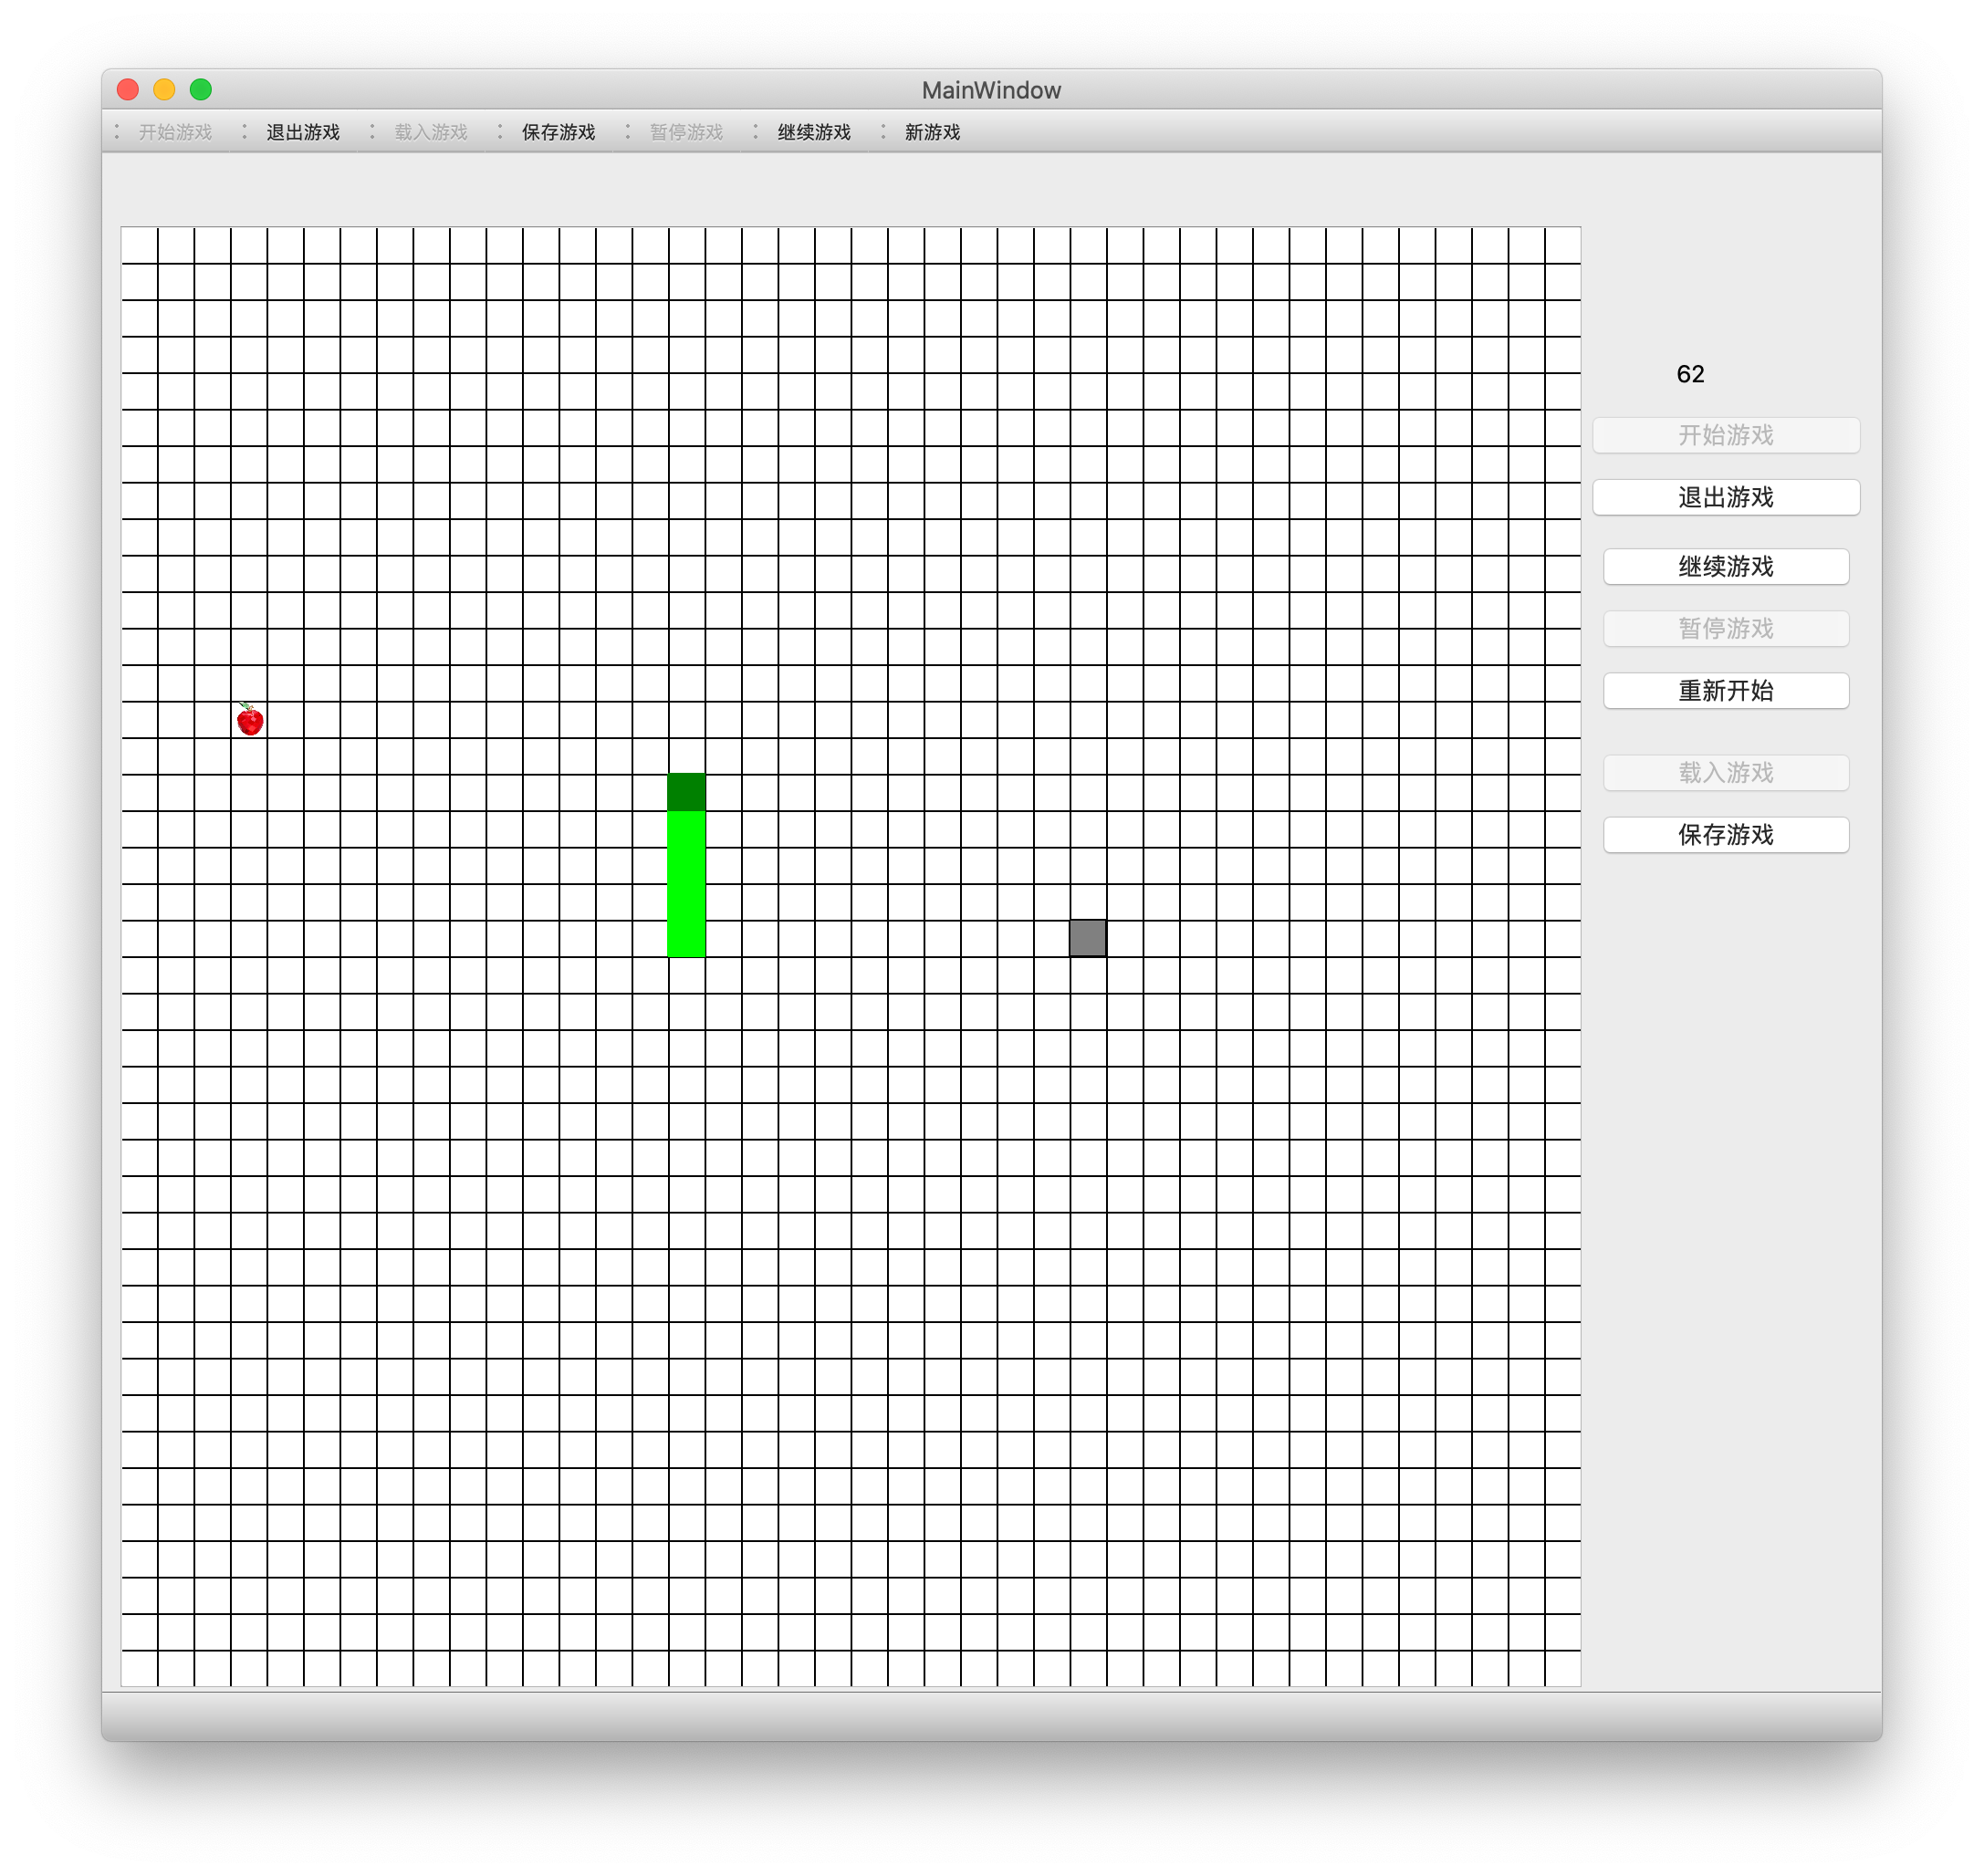
\includegraphics[scale = 0.2]{texsrc/界面paused.png}
        \caption{暂停状态}
        \label{paused}
    \end{figure}
    \paragraph{暂停状态} 当在游戏过程中选择暂停或者重新载入了已有的游戏后,将进入暂停状态(图4)。此时蛇将停止移动,计时器也停止计时。此时开始游戏、暂停游戏、载入游戏三个功能
    将无法使用。
    \par 此时点击继续游戏将进入游戏状态,继续工作;此时点击保存游戏可以导出此游戏,保存为.txt文件,文件格式见下。

    \subsection{游戏保存文件}

    \section{程序架构}
    \subsection{实现方案}
    程序实现了5个类:MainWindow、gamecontroller、food、obstacles、snake。其中MainWindow负责显示界面,
    gamecontroller主要负责游戏的逻辑和控制,并且记录了当前用户所处的状态,
    food、obstacles、snake三类分别实现了食物、障碍、蛇的运动记录、绘制等功能。
    在程序内部储存位置时,都以行、列数的虚拟坐标进行储存,并定义了由行、列坐标与scene中坐标互相转化的方法。
    \subsection{MainWindow类}
    MainWindow类就是创建程序时自动创建的主窗口类,主要负责进行程序界面的设计并实现有关组件展示内容、样式的方法。
    \paragraph{数据成员}
    \begin{lstlisting}
        Ui::MainWindow *ui;
        /*--所有操作对应的QAction--*/
        QAction* start;
        QAction* quit;
        QAction* load;
        QAction* save;
        QAction* pause;
        QAction* restart;
        QAction* unpause;
        /*--游戏界面--*/
        QGraphicsView* view;
        QGraphicsScene* scene;
        /*--游戏的控制器 game--*/
        gamecontroller* game;
    \end{lstlisting}
    \paragraph{实现接口}
    \begin{lstlisting}
        /*-构造与析构函数,负责窗口的初始化-*/
        MainWindow(QWidget *parent = nullptr);
        ~MainWindow();
        /*-窗口组件相关功能-*/
        void setButtonsStatus();//根据当前状态设置按键和QAction的状态
        void setView();//设置游戏窗口大小
        void initBackground();//根据行、列数初始化游戏窗口的网格
        void setDisplayTime(int time = 0);//设置时间展示组件的时间
        /*-事件过滤器,为游戏窗口安装-*/
        bool eventFilter(QObject* object, QEvent* event) override;
    \end{lstlisting}
    \subsection{gamecontroller类}
    gamecontroller类负责控制整个游戏,实现了控制各类的函数,并且设定了状态的枚举类
    \paragraph{数据成员}
    \begin{lstlisting}
        gameStatus status = gameStatus::initialized;//游戏当前状态

        MainWindow* father;//MainWindow成员
        QTimer* timer;//用于进行时间循环的QTimer
        QGraphicsScene* scene;//场景
        food* apple;//当前游戏的食物
        snake* Snake;//当前游戏的蛇
        QMap<Pii,obstacles*> barrier;//当前游戏的所有
        int time = 0;//蛇运行的步数
    \end{lstlisting}
    \paragraph{实现接口}
    \begin{lstlisting}
        /*-当进行了一定操作的时候调用的方法-*/
        void pause();
        void start();
        void restart();
        void load();
        void save();
        void resume();
        void gamelost();//游戏结束方法
        /*-处理输入的方法-*/
        void handleClick(Pii a);//处理鼠标点击的方法
        void handlePress(QKeyEvent*);//处理键盘按键的方法
        /*-游戏运行中调用的方法-*/
        void handleSnakeCollide();//在刷新场景前判断蛇的碰撞,并进行相应的处理
        void handleSnakeEating();//当蛇吃苹果后的方法
        void setNewFood();//放置一个新的水果
        gamecontroller::gameStatus getStatus();//返回当前游戏的状态
        advance();//每次更新当前状态的方法
    \end{lstlisting}
    \subsection{food、obstacles、snake类}
    这三个类是场景中的物体类,继承自QGraphicsItem,重新实现了画图函数;
    其中snake类还重新实现了advance()函数,用以更新snake对象的位置,实现移动功能;同时也实现了增长的功能。
\end{document}